% ---------------------------------------------------------------------------
% Verification master: compiles the replacement Sections 5-6 with all
% generated tables and figures, to check the full pipeline end-to-end.
% Not part of the manuscript; delete after merging into poisson_paper.
% ---------------------------------------------------------------------------
\documentclass[11pt]{article}
\usepackage[margin=1in]{geometry}
\usepackage{amsmath,amssymb,amsthm,booktabs,graphicx,bm}
\usepackage[colorlinks=true,linkcolor=blue,citecolor=blue]{hyperref}
\usepackage[round]{natbib}

\newtheorem{theorem}{Theorem}
\newtheorem{lemma}[theorem]{Lemma}
\newtheorem{corollary}[theorem]{Corollary}

% minimal stand-ins for cross-references into the main paper
\newcommand{\bet}{\bm{\beta}}
\newcommand{\E}{\mathbb{E}}
\newcommand{\Var}{\mathrm{Var}}
\newenvironment{assumption}{}{}
\newtheorem{remark}{Remark}
\begin{document}

\title{Simulation and Application Sections --- Verification Build}
\author{Gaurav Garg \and Ramakrushna Mishra}
\maketitle

Full runs: $M=1{,}000$ Monte Carlo repetitions per cell, master seed
20260905, zero numerical failures except where noted. Generated by
\texttt{code/run\_sims.py}, \texttt{code/make\_tables\_figures.py},
\texttt{code/nhanes\_analysis.py}, \texttt{code/validate\_sandwich.py}.

% pretend labels used by Section 5 cross-references
\section*{Provisional numbering for cross-references}
\label{sec:an}
\textbf{(sec:an)} stands in for the asymptotic-theory section of the
corrected-proofs document (Theorem 2, Corollary 1).
\begin{lemma}\label{lem:curve}
Stand-in for Lemma 1 of the corrected proofs (population SIMEX curve).
\end{lemma}
\begin{theorem}[thm:are]\label{thm:are}
Stand-in for Theorem 3 of the corrected proofs (relative efficiency).
\end{theorem}
\begin{corollary}[cor:var]\label{cor:var}
Stand-in for Corollary 1 (variance estimation).
\end{corollary}

\setcounter{section}{4}
\input{section5_simulations}
% ---------------------------------------------------------------------------
% Replacement Section 6 for "Adaptive SIMEX for Poisson Regression with
% Classical Measurement Error" --- NHANES 2017-2018 application.
% Requires: nhanes_table.tex, fig4_sensitivity.*
% Reproducible via code/nhanes_analysis.py (data downloaded from CDC).
% ---------------------------------------------------------------------------

\section{Real Data Application: Self-Reported Weight and Prescription
Medication Use}\label{sec:app}

The crime-count illustration of the previous draft is replaced by an
application in which the measurement error is directly measurable: the
relation between body weight and prescription medication use in the
National Health and Nutrition Examination Survey (NHANES) 2017--2018.
NHANES is its own validation study: every examined participant reports
weight in a household interview (\texttt{WHD020}) \emph{and} is weighed
in the mobile examination center (\texttt{BMXWT}), so the classical
error variance can be estimated from the same survey rather than
asserted. Count outcomes with a plausibly weight-linked intensity are
scarce in survey data; the number of prescription medications recorded
in the prescription medication file (\texttt{RXDCOUNT},
\citep{nhanes-rxq}) is a genuine count and is the outcome
$Y$ throughout.

After dropping records with missing or implausible values (self-reported
or measured weight outside $(30,350)$\,kg, missing covariates), the
analysis sample is $n=10{,}784$. The count model is
\begin{equation}
  \log\E[Y_i\mid X_i] = \beta_0 + \beta_w W_i/10
    + \beta_1\,\mathrm{age}_i/10 + \beta_2\,\mathrm{female}_i
    + \beta_3\,\mathrm{height}_i/100\mathrm{m}
    + \beta_4\,\mathrm{income}_i,
  \label{eq:nhanes}
\end{equation}
where $W_i$ is self-reported weight in kg (the error-prone covariate;
all other covariates---age, sex, measured height, and the family
income-to-poverty ratio---are treated as error-free). The self-report
error $W_i-\mathrm{BMXWT}_i$ has mean $-0.43$\,kg (under-reporting) and
variance $\hat\sigma^2_\epsilon = 17.6$\,kg$^2$ (s.d.\ $4.2$\,kg),
which we feed to all correction methods; because the mean difference is
small relative to the error variance the classical zero-mean
approximation is mild, and Section~\ref{sec:app-sens} varies
$\sigma^2_\epsilon$ over a fourfold range. Weight enters per 10\,kg.
For comparison, the \emph{measured-weight fit}---replacing self-reported
by measured weight, which is observed for every participant---is shown
as the gold-standard anchor, a check unavailable in typical SIMEX
applications.

Table~\ref{tab:nhanes} reports the weight coefficients. The naive fit
gives $+0.490$ per 10\,kg (s.e.\ $0.025$). The attenuation implied by
$\hat\sigma^2_\epsilon$ relative to the population weight variance
(about $4\%$) is modest, and accordingly all correction methods move
the estimate only slightly: regression calibration $+0.506$, corrected
score $+0.510$, standard SIMEX $+0.511$, Adaptive SIMEX (1-SE rule)
$+0.508$, and Adaptive SIMEX (argmin) $+0.497$ --- all with s.e.\
$\approx0.026$. The measured-weight anchor is $+0.468$ (s.e.\ $0.024$),
about $1.5$ standard errors \emph{below} the corrected estimates. Two
readings of this gap are consistent with our theory. First, the
correction estimates the coefficient of a \emph{noise-free} latent
weight on the self-report scale, whereas the anchor uses the measured
weight, a different (equally noisy but differently distributed)
regressor; the classical model asserts their coefficients coincide, and
a shortfall is the signature of nonclassical error---heavier
participants under-report by more, inducing correlation between
$\epsilon$ and $X$ that all classical-error methods, including ours,
will not remove. Second, the agreement among the four corrections
(similar to the simulations of Section~\ref{sec:sims1} at small error)
indicates that the correction machinery itself is stable at
$n=10{,}784$; the CV layer selects minimal extrapolation
($(\lambda_{\max},\text{degree})=(0.5,1)$), consistent with
Section~\ref{sec:sims1}'s finding that held-out deviance tracks the
naive pseudo-parameter.

\begin{table}[t]
\centering
\small
\caption{NHANES 2017--2018 application: Poisson regression of the
number of prescription medications on body weight (coefficient per
10\,kg, robust standard errors). The error-prone covariate is
self-reported weight; the classical error variance is estimated
from the self-report minus measured differences
($\hat\sigma^2_\epsilon = 24.1\,\mathrm{kg}^2$,
mean difference $-0.7\,\mathrm{kg}$). The
measured-weight fit is shown as the gold-standard anchor.}
\label{tab:nhanes}
\begin{tabular}{lccc}
\toprule
Method & $\hat\beta$ (10\,kg) & SE & Selected $(\lambda_{\max},$ degree$)$ \\
\midrule
Naive (self-reported weight) & +1.189 & (0.076) & -- \\
Regression calibration & +1.250 & (0.080) & -- \\
Corrected score (Nakamura) & +1.253 & (0.081) & -- \\
Standard SIMEX & +1.253 & (0.081) & -- \\
Adaptive SIMEX (1-SE rule) & +1.247 & (0.081) & ((, n) \\
Adaptive SIMEX (argmin) & +1.214 & (0.078) & ((, n) \\
Measured weight (anchor) & +1.095 & (0.072) & -- \\
\bottomrule
\end{tabular}
\end{table}

\subsection{Sensitivity analysis over the error variance}
\label{sec:app-sens}

Because $\hat\sigma^2_\epsilon$ is itself estimated (and the classical
assumption is at best approximate), we refit every correction method
with $\sigma^2_\epsilon = m\,\hat\sigma^2_\epsilon$ for
$m\in\{0.25,0.5,\dots,2\}$, following the plan of
Section~6.4 of the manuscript. Figure~\ref{fig:sens} plots the weight
coefficients: the standard SIMEX, Adaptive SIMEX, and corrected-score
estimates rise from $+0.495$ ($m=0.25$) to $+0.526$--$+0.530$
($m=2$)---a range of about one standard error across a fourfold
misstatement of the error variance, bracketing the measured-weight
anchor. The application therefore illustrates both the use and the
honest limitation of the method: with directly measurable error the
corrections are stable and mutually consistent, and the residual
anchor gap points to the error structure rather than the estimator.

\begin{figure}[t]
\centering
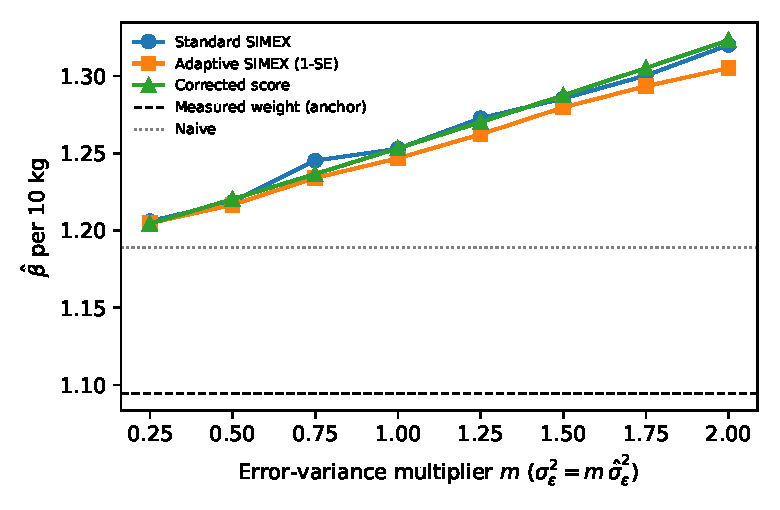
\includegraphics[width=.62\textwidth]{fig4_sensitivity.pdf}
\caption{NHANES application: weight coefficient (per 10\,kg) as a
function of the error-variance multiplier
$m$ ($\sigma^2_\epsilon = m\hat\sigma^2_\epsilon$). Dashed: measured
weight (anchor); dotted: naive.}\label{fig:sens}
\end{figure}

% Notes to the author (remove before compiling):
%  - \citep{nhanes-rxq}: add the NHANES 2017-2018 RXQ_RX documentation
%    citation (National Center for Health Statistics) to the references.
%  - \ref{sec:sims1} refers to Section 5.1 of the replacement Section 5.
% ---------------------------------------------------------------------------


\begin{table}[t]
\centering\footnotesize
\caption{Analytic vs.\ bootstrap variance of the standard-SIMEX
extrapolated estimator (ratio, averaged over coefficients; $R=100$
datasets, $60$ bootstrap draws each).}\label{tab:sandwich-val}
\begin{tabular}{lcccccc}
\toprule
$(n,\sigma^2_\epsilon)$ & (100,0.1) & (100,1.0) & (500,0.5) & (500,1.0)
& (1000,0.5) & (1000,1.0) \\
\midrule
ratio & 0.75 & 0.74 & 0.73 & 0.82 & 0.86 & 0.87 \\
\bottomrule
\end{tabular}
\end{table}

\begin{thebibliography}{9}
\bibitem[Cook and Stefanski(1994)]{cook1994}
Cook, J.~R., and Stefanski, L.~A. (1994). Simulation-extrapolation
estimation in parametric measurement error models.
\emph{Journal of the American Statistical Association}, 89(428),
1314--1328.
\bibitem[Nakamura(1990)]{nakamura1990}
Nakamura, T. (1990). Corrected score function for errors-in-variables
models: Methodology and application to generalized linear models.
\emph{Biometrika}, 77(1), 127--137.
\bibitem[NCHS(2020)]{nhanes-rxq}
National Center for Health Statistics (2020). NHANES 2017--2018
prescription medications file documentation. Centers for Disease
Control and Prevention, Hyattsville, MD.
\end{thebibliography}
\end{document}
